%!TEX root = ../../main.tex

\chapter{Das Monty-Hall-Problem}

\section{Einführung}

Das Monty-Hall-Problem (oft auch als Ziegenproblem bezeichnet) ist Statistikern als Paradoxon in der Elementarwahrscheinlichkeitstheorie bekannt. Es geht dabei um die Frage, ob eine Wahl, die zunächst
zufällig unter drei a priori gleich wahrscheinlichen Möglichkeiten getroffen wurde, geändert werden sollte, wenn zusätzliche
Informationen enthüllt werden. Die Aufgabe ist ursprünglich aus der von Monty Hall modertierten Spielshow ,,Lets Make a Deal'' abzuleiten. Sie fand ihren Anfang
1963 und ihr Ende 1977. In jeder Folge spielte der Moderator der Spielshow, Monty Hall, Spiele mit seinem Publikum. Diese Spiele variierten stark, jedoch war das Grundprinzip
häufig das Selbe. Spieler aus dem Publikum mussten sich zwischen garantierten, kleinen Gewinnen und eventuellen, durch ,,Glückspiel'' gewonnene, große Preise, entscheiden.
In einer der Folgen, die häufig als die Klimax der Show beschrieben wird, wurde den Spielern aus dem Publikum drei identische Türen gezeigt. Hinter diesen drei
identischen Türen befinden sich die potenziellen Gewinne, wovon zwei Gewinne Ziegen waren. Hinter der dritten Tür war jedoch der Hauptgewinn, ein neues Auto.

Das Problem, wie es heutzutage unter Mathematikern bekannt ist, wurde ursprünglich als Leserbrief an Marilyn vos Savant (oft ,,die Klügste Frau der Welt genannt'') in ihrer Kolumne \textit{Ask Marilyn} im Magazin Parade veröffentlicht:

\begin{quote}
    Nehmen Sie an, Sie wären in einer Spielshow und hätten die Wahl zwischen drei Toren. Hinter einem der Tore ist ein Auto, hinter den anderen sind Ziegen. Sie wählen ein Tor, sagen wir, Tor Nummer 1, und der Showmaster, der weiß, was hinter den Toren ist, öffnet ein anderes Tor, sagen wir, Nummer 3, hinter dem eine Ziege steht. Er fragt Sie nun: ,,Möchten Sie das Tor Nummer 2?'' Ist es von Vorteil, die Wahl des Tores zu ändern? (\cite{Savant:1990})
\end{quote}

Dieses Problem zeigt, wie die intuitive Wahrnehmung von Wahrscheinlichkeiten von der tatsächlichen Mathematik abweichen kann. Selbst unter Mathematikern wurde das Problem und vor allem die von vos Savant vorgestellte Lösung stark diskutiert und kritisiert\footnote{wie wir später sehen werden nicht ganz zu Unrecht}.

\section{Möglichkeiten des Kandiaten}

Grundlegend hat der Kandidat nachdem der Moderator ein Ziegentor geöffnet hat: Wechseln oder nicht wechseln. Die meisten, die sich vorher noch nicht mit diesem Problem beschäftigt haben, werden intuitiv denken, dass sie hier eine Gewinnwahrscheinlichkeit von $50\%$ haben, egal ob sie wechseln oder nicht. Andere denken womöglich, der Moderator möchte einem dazu bringen, die Auswahl zu ändern, da sie mit ihrer ersten Wahl richtig lagen.

\subsection{Wechseln oder nicht ist egal}

Zu diesem Schluss kommen die meisten, wenn sie sich das erste Mal mit diesem Problem auseinandersetzen. Sie gehen davon aus, dass sie nun eine Gewinnwahrscheinlichkeit von $50\%$ haben, egal wie sie sich entscheiden.

\subsection{Bei der ersten Wahl bleiben}

Geht man davon aus, bei beiden Toren die gleiche Gewinchance zu haben, entscheiden sich die meisten dafür, bei ihrer ersten Wahl zu bleiben. Dies lässt sich damit erklären, dass man von einer einmaligen Spielsituation ausgeht (im Leserbrief wurde auch nichts anderes erwähnt) und man nichts über die Motivation des Moderators weiß. Wenn man schon einige Spielshows gesehen hat, denkt man möglicherweiße aus Erfahurung, der Moderator wolle einen nur verunsichern und von der ersten richtigen Wahl abbringen.\footnote{Dass die meisten bei ihrer Ursprünglichen Wahl bleiben, wurde genauer in der Dokuserie ,,Mythbusters'' (Staffel 9, Episode 21) untersucht und bestätigt.}

\subsection{Auf jeden Fall wechseln}

Nur die wenigsten treffen diese Wahl.

\section{Die Lösung}

Doch die Lösung von vos Savos sagt, man hätte eine Gewinnchance von \sfrac{2}{3} wenn man wechselt während man bei der ursprünglichen Wahl nur in \sfrac{1}{3} der Fälle das Auto gewinnt:

\begin{quote}
    Ja; Sie sollten wechseln. Das erste Tor hat eine Chance von \sfrac{1}{3} zu gewinnen, aber das Zweite hat eine \sfrac{2}{3} Chance. Hier ist eine gute Möglichkeit um darzustellen was passiert ist. Angenommen es gäbe eine millionen Tore, und Sie wählen Tor 1. Dann öffnet der Host, der weiß was hinter jedem Tor ist und immer das Tor mit dem Gewinn vermeidet, alle Tore außer das Tor mit der Nummer 777777. Sie würden direkt wechseln, oder? (\cite{Savant:1990})
\end{quote}

Anders erklärt kann man auch folgendermaßen Argumentieren: Dass der Kandidat auf Anhieb das richte Tor erwischt liegt bei der A-priori-Wahrscheinlichkeit von \sfrac{1}{3} und dass das Auto hinter einem der anderen Tore steht bei \sfrac{2}{3}. Wird nun ein Tor geöffnet, kann sich die Wahrscheinlichkeit, dass die erste Wahl richtig war nicht geändert haben. Dadurch liegen die Wahrscheinlickeiten der übrigen Tore nicht bei \sfrac{1}{2}, sondern hinter dem Tor, das nicht zuerst gewählt war und nicht vom Moderator geöffnet wurde, steht mit einer Wahrscheinlichkeit von \sfrac{2}{3} das Auto.

Der Entscheidungsbaum in \ref{fig:tree} veranschaulicht alle Fäll, bei denen das Auto hinter dem ersten Tor steht. Bei den Fällen (1) und (2) gewinnt man, wenn man nicht wechselt, mit Wechseln gewinnt man in den Fällen (3) und (4). Addiert man die Wahrscheinlichkeiten der jeweiligen Pfade erhällt man die Gewinnwahrscheinlichkeiten für Wechseln ($P_W$) und Bleiben ($P_B$):

\begin{equation}
    \begin{split}
        P_W & = P(T_1T_2) + P(T_1T_3) \\
        & = \frac{1}{6} + \frac{1}{6} = \frac{1}{3} \\
        P_G & = P(T_2T_3) + P(T_3T_2) \\
        &= \frac{1}{3} + \frac{1}{3} = \frac{2}{3} \\
    \end{split}
\end{equation}

Somit haben wir die Lösung von vos Savos bestätigt.

\begin{figure}[htbp]
    \centering
    \fbox{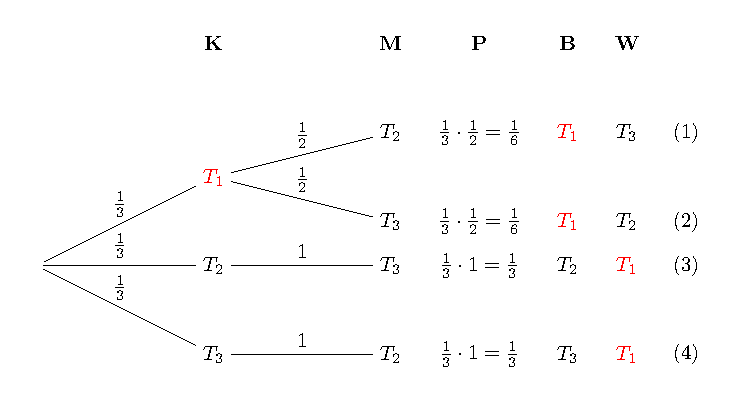
\includegraphics{tex/tree.pdf}}
    \caption{Entscheidungsbaum}\label{fig:tree}
    \small {Der Baum stellt den Ablauf der Spieleshow für den Fall, dass hinter dem ersten Tor ($T_1$) das Auto steht, dar. Zunächst trifft der Kandidat seine erste Wahl (K). Anschließend öffnet der Moderator ein Ziegentor, dass nicht vom Kandidaten gewählt wurde (M). Entlag der Pfade werden die Wahrscheinlicketen mutipliziert (P). (B) und (W) zeigen die Tore, die man beim Bleiben bzw. beim Wechseln öffnen würde.}
\end{figure}
